% ---------------------------------------------------------------------------
% Informe del Proyecto 1 -- Curso de NLP
% DistilBERT vs BERT en clasificacion de texto
%
% Compilar:  make            (usa tectonic)
%            tectonic -X compile main.tex
%
% Las figuras NO se copian aqui: se leen de ../../results/figures/, que es
% donde las escribe `python -m src.plots`. Asi el informe nunca muestra una
% version vieja de una figura que ya se regenero.
% ---------------------------------------------------------------------------
\documentclass[11pt,a4paper]{article}

\usepackage[T1]{fontenc}
\usepackage[utf8]{inputenc}
\usepackage[spanish,es-noquoting,es-tabla]{babel}
\usepackage[margin=2.5cm]{geometry}
\usepackage{graphicx}
\usepackage{booktabs}
\usepackage{siunitx}
\usepackage{amsmath}
\usepackage{caption}
\usepackage{subcaption}
\usepackage{xcolor}
\usepackage{enumitem}
\usepackage{listings}
\usepackage[hidelinks]{hyperref}

% Las figuras vienen del pipeline; el segundo camino permite distribuir la
% carpeta del informe por separado copiando las figuras dentro.
\graphicspath{{../../results/figures/}{figuras/}}

% babel-spanish reconfigura siunitx al cargarse, asi que un \sisetup en el
% preambulo se pierde: con el separador por defecto, 109483778 salia como
% "109,483,778" con la misma coma que el separador decimal ("0,9232"), y
% ademas \num{0.9232} se agrupaba como "0,923,2". Aplicado al inicio del
% documento, la configuracion es la ultima en ejecutarse y gana.
\AtBeginDocument{\sisetup{
  output-decimal-marker = {,},
  group-separator       = {\,},   % espacio fino: no se confunde con la coma
  group-digits          = integer, % nunca agrupar la parte decimal
  group-minimum-digits  = 4,
  detect-weight         = true,
}}

% Los identificadores largos en \texttt (ClasificadorConCabeza,
% AutoModelForSequenceClassification) no se pueden partir, y en un parrafo
% justificado desbordan el margen. emergencystretch deja a TeX estirar los
% espacios de esas lineas en lugar de salirse.
\setlength{\emergencystretch}{3em}

\captionsetup{font=small, labelfont=bf, width=0.92\textwidth}
\setlist[itemize]{itemsep=2pt, topsep=4pt}
\setlist[enumerate]{itemsep=2pt, topsep=4pt}

\definecolor{codebg}{HTML}{F4F4F1}
\lstset{
  basicstyle=\ttfamily\footnotesize,
  backgroundcolor=\color{codebg},
  frame=none, breaklines=true, columns=fullflexible, keepspaces=true,
  xleftmargin=8pt, framexleftmargin=8pt, aboveskip=8pt, belowskip=8pt,
  literate={á}{{\'a}}1 {é}{{\'e}}1 {í}{{\'i}}1 {ó}{{\'o}}1 {ú}{{\'u}}1 {ñ}{{\~n}}1,
}

\newcommand{\best}[1]{\textbf{#1}}

\title{\vspace{-1.5cm}\textbf{DistilBERT frente a BERT en clasificación de texto}\\[2pt]
       \large Desempeño, eficiencia y un estudio de ablación sobre tres datasets}
\author{Proyecto 1 --- Curso de Procesamiento de Lenguaje Natural}
\date{}

\begin{document}
\maketitle

\section*{Resumen}
\addcontentsline{toc}{section}{Resumen}

Se hizo \textit{fine-tuning} de BERT-base y DistilBERT-base sobre tres tareas
de clasificación de texto (SST-2, AG News y Yelp Polarity) bajo un protocolo
idéntico, y se comparó a los dos modelos en desempeño y en eficiencia. Sobre
esa base se ejecutó un estudio de ablación de seis configuraciones que varía
la cabeza de clasificación y qué parte del \textit{transformer} se entrena.

Los resultados sostienen tres afirmaciones. Primera: con el \SI{61}{\percent}
de los parámetros, DistilBERT conserva entre el \SI{98,9}{\percent} y el
\SI{99,5}{\percent} de la \textit{accuracy} de BERT, y la brecha depende de la
tarea --- se abre en análisis de sentimiento sobre frases cortas y se cierra
hasta desaparecer en clasificación de temas. Segunda: medida en condiciones
comparables, la inferencia de DistilBERT es exactamente \best{2$\times$} más
rápida en los nueve puntos de una rejilla de \textit{batch} y longitud, que es
lo que predice pasar de 12 capas a 6. Tercera: la arquitectura de la cabeza de
clasificación es irrelevante --- cinco configuraciones distintas caben en
\num{0,0014} de F1 --- mientras que congelar el \textit{encoder} cuesta entre
\num{3,4} y \num{8,4} puntos de F1 según la tarea.

En total son \num{24} corridas de entrenamiento, unas \num{2,5} horas de GPU
en una NVIDIA RTX A6000. Todas las métricas de este informe se generan
automáticamente desde los archivos JSON versionados en el repositorio.


{\small\tableofcontents}
\vspace{0.6cm}
\section{Introducción y objetivos}

BERT \cite{devlin2019bert} estableció el procedimiento estándar para tareas
de clasificación de texto: pre-entrenar un \textit{transformer} bidireccional
sobre texto no etiquetado y después ajustarlo a la tarea concreta. El costo de
ese procedimiento, sin embargo, es alto en inferencia, que es donde un modelo
pasa la mayor parte de su vida útil. DistilBERT \cite{sanh2019distilbert}
responde a ese costo con destilación de conocimiento: un modelo de 6 capas
entrenado para imitar a uno de 12, con la promesa de conservar la mayor parte
del desempeño a la mitad del tamaño.

Este proyecto pone esa promesa a prueba con una condición que se respeta en
todo el trabajo: \textbf{la única diferencia entre las dos columnas de
cualquier tabla debe ser el modelo}. Mismo código, mismos datos, mismo
optimizador, misma semilla, misma GPU. Cuando esa condición no se puede
cumplir --- y hay un caso en el que no se cumple, la latencia medida al final
de cada entrenamiento --- se dice explícitamente y se mide de nuevo en
condiciones controladas (Sección~\ref{sec:eficiencia}).

Los objetivos concretos son cuatro:

\begin{enumerate}
  \item Ajustar ambos modelos a tres tareas de clasificación de distinta
        naturaleza y tamaño, bajo un protocolo idéntico.
  \item Reportar el desempeño con \textit{accuracy}, \textit{precision},
        \textit{recall} y F1, y la eficiencia con número de parámetros,
        latencia de inferencia y memoria de GPU.
  \item Determinar, mediante un estudio de ablación, qué partes del modelo
        contribuyen realmente al desempeño: la arquitectura de la cabeza de
        clasificación o la adaptación del \textit{encoder}.
  \item Aplicar la configuración ganadora a ambos modelos y comparar.
\end{enumerate}

\section{Datos}
\label{sec:datos}

Se eligieron tres tareas que varían en número de clases, longitud de texto y
tamaño, para que las conclusiones no dependan de un único régimen: SST-2
\cite{socher2013sst}, distribuida dentro del \textit{benchmark} GLUE
\cite{wang2019glue}, y AG News y Yelp Polarity, ambas en la recopilación de
Zhang et al.\ \cite{zhang2015character}.

\begin{table}[h]
\centering
\small
\begin{tabular}{llcrrrc}
\toprule
\textbf{Dataset} & \textbf{Fuente (HuggingFace)} & \textbf{Clases} &
\textbf{Train} & \textbf{Val.} & \textbf{Test} & \textbf{\texttt{max\_length}} \\
\midrule
SST-2          & \texttt{nyu-mll/glue}, conf.\ \texttt{sst2} & 2 & \num{60614}  & \num{6735}  & \num{872}   & 64  \\
AG News        & \texttt{fancyzhx/ag\_news}                  & 4 & \num{108000} & \num{12000} & \num{7600}  & 128 \\
Yelp Polarity  & \texttt{fancyzhx/yelp\_polarity}            & 2 & \num{100000}$^{*}$ & \num{20000}$^{*}$ & \num{38000} & 256 \\
\bottomrule
\end{tabular}
\caption{Los tres datasets, ya normalizados por \texttt{src/data\_adapter.py}.
($^{*}$) Yelp va submuestreado; véase más abajo.}
\end{table}

\subsection{Normalización}

Los tres datasets llegan del Hub con esquemas distintos: SST-2 llama
\texttt{sentence} a su columna de texto y arrastra una columna \texttt{idx};
AG News y Yelp usan \texttt{text}; ninguno de los tres trae los mismos splits.
El módulo \texttt{src/data\_adapter.py} los reduce a una forma única --- un
\texttt{DatasetDict} con splits \texttt{train}/\texttt{validation}/\texttt{test}
y solo las columnas \texttt{text} (str) y \texttt{label} (int) --- de modo que
el resto del \textit{pipeline} no sabe con qué dataset trabaja. Añadir una
tarea nueva es añadir una entrada a un registro, no tocar el entrenamiento.

\subsection{Dos decisiones sobre los splits}

Ambas afectan a cómo deben leerse los números, así que conviene dejarlas
explícitas.

\paragraph{El \texttt{test} de SST-2 no se usa.} En GLUE ese split viene sin
etiquetas (\texttt{label = -1}), porque la evaluación oficial es en servidor.
Se usa entonces el \texttt{validation} oficial (\num{872} frases) como
conjunto de test, y se aparta un \SI{10}{\percent} del train como validación
propia. Es el protocolo habitual en la literatura, y es lo que hace que
nuestros números sean comparables con los publicados. El adaptador verifica
explícitamente que ningún split contenga la etiqueta $-1$ y aborta si la
encuentra: es la clase de error que, si pasa inadvertido, produce métricas sin
sentido sin lanzar ninguna excepción.

\paragraph{Yelp va submuestreado.} Se usan \num{100000} de las \num{560000}
reseñas de train y \num{20000} de validación. Entrenar con el conjunto
completo a 256 \textit{tokens} multiplicaría por cinco el costo para mover la
\textit{accuracy} algunas décimas. Lo importante para la validez de la
comparación es que \textbf{el mismo presupuesto se aplica a los dos modelos}:
el submuestreo usa la misma semilla y produce exactamente el mismo
subconjunto para BERT y para DistilBERT.

En los dos datasets que no traen un split de validación etiquetado (AG News y
Yelp), la validación es un \SI{10}{\percent} del train separado con semilla
fija. El conjunto de test nunca participa en ninguna decisión.

\section{Metodología}
\label{sec:metodologia}

\subsection{Los modelos y qué se hizo con los pesos}
\label{sec:pesos}

Esta subsección es deliberadamente explícita, porque el tratamiento de los
pesos pre-entrenados es donde un experimento de \textit{fine-tuning} se
invalida con más facilidad y sin dar ningún error.

\paragraph{Origen.} Los dos modelos se construyen a partir de los
\textit{checkpoints} públicos de HuggingFace, que se enumeran en la
Tabla~\ref{tab:modelos}. DistilBERT es una destilación del primero de ellos:
conserva una de cada dos capas, elimina el \textit{pooler} y los
\textit{embeddings} de segmento, y mantiene la dimensión oculta (768) y el
vocabulario. Los pesos se descargan del Hub en el momento de construir el
modelo; \textbf{no hay ningún peso almacenado en el repositorio}, ni
versionado, ni modificado, ni redistribuido. El repositorio contiene
únicamente código, métricas en JSON y figuras.

\begin{table}[h]
\centering
\small
\begin{tabular}{llcr}
\toprule
\textbf{Nombre corto} & \textbf{\textit{Checkpoint} en el Hub} &
\textbf{Capas} & \textbf{Parámetros} \\
\midrule
BERT-base       & \texttt{bert-base-uncased}       & 12 & \num{109483778} \\
DistilBERT-base & \texttt{distilbert-base-uncased} &  6 & \num{66955010}  \\
\bottomrule
\end{tabular}
\caption{Los dos \textit{checkpoints} de partida. El número de parámetros
corresponde a una cabeza de dos clases; con las cuatro clases de AG News
sube en \num{1538} en ambos modelos ($768 \times 2 + 2$ pesos de salida
adicionales).}
\label{tab:modelos}
\end{table}

\paragraph{Qué se inicializa al azar.} Al construir un clasificador, el
\textit{encoder} llega pre-entrenado pero la cabeza de clasificación se
inicializa aleatoriamente: es la única parte que no ha visto nunca datos. El
aviso \textit{``newly initialized''} que imprime \texttt{transformers} es
esperado y correcto; su ausencia sería la señal de alarma. La semilla 42 fija
esa inicialización, de modo que la cabeza de BERT y la de DistilBERT parten
del mismo estado aleatorio.

\paragraph{Qué se actualiza durante el entrenamiento.} En las corridas base
se actualizan todos los parámetros: \textit{encoder} y cabeza. En las
configuraciones congeladas del estudio de ablación se pone
\texttt{requires\_grad = False} sobre el \textit{encoder} y, además, esos
parámetros \textbf{no se pasan al optimizador}. Los dos pasos son necesarios:
con solo el primero, AdamW seguiría aplicando \textit{weight decay} a pesos
que no reciben gradiente, y el modelo se degradaría de forma silenciosa.

\paragraph{El tokenizador se deriva siempre del modelo.} Cada
\textit{checkpoint} trae su propio vocabulario. Usar el tokenizador de otro
modelo rompe la correspondencia entre \textit{token} e \textit{embedding} y
el modelo predice ruido sin lanzar ninguna excepción. Por eso
\texttt{build\_tokenizer()} nunca acepta un vocabulario suelto: lo deriva del
identificador del modelo.

\paragraph{Qué se conserva y qué no.} Durante el entrenamiento se mantiene en
memoria una copia del \textit{state dict} de la época con mejor F1 de
validación, y es esa copia la que se carga antes de evaluar en test. Al
terminar, el modelo ajustado \textbf{se descarta}: no se escribe en disco ni
se versiona. Todo lo que sobrevive a una corrida son sus métricas. Es una
decisión consciente --- los \textit{checkpoints} ajustados pesan cientos de
megabytes cada uno y son reproducibles desde el código y la semilla --- y
tiene la consecuencia práctica de que cargar de nuevo cualquier modelo del
proyecto parte siempre de los pesos originales del Hub, sin estados
intermedios que puedan haberse corrompido.

\subsection{La cabeza de clasificación del estudio de ablación}

Las clases \texttt{AutoModelForSequenceClassification} de HuggingFace traen
una cabeza fija, y --- esto es lo que obliga a no usarlas aquí --- una cabeza
\textbf{distinta en cada arquitectura}: BERT pasa el \textit{token}
\texttt{[CLS]} por un \textit{pooler} con \texttt{tanh}; DistilBERT usa un
\texttt{pre\_classifier} con \texttt{ReLU}. Comparar cabezas montadas sobre
dos preprocesos distintos mezclaría dos variables en el mismo experimento.

Por eso el estudio de ablación usa una envoltura propia
(\texttt{ClasificadorConCabeza} en \texttt{src/models.py}): \textit{encoder}
desnudo (\texttt{AutoModel}) más un MLP construido por nosotros sobre el
estado oculto del \textit{token} \texttt{[CLS]}, idéntico para las dos
arquitecturas. Así la única diferencia entre dos corridas es lo que el
experimento cambia a propósito.

\subsection{Protocolo de entrenamiento}

El bucle de entrenamiento está escrito a mano, sin el \texttt{Trainer} de
HuggingFace, para tener control explícito sobre el \textit{scheduler}, el
recorte de gradientes y el registro por iteración. Los hiperparámetros son
idénticos para los dos modelos y las tres tareas.

\begin{table}[h]
\centering
\small
\begin{tabular}{ll}
\toprule
Optimizador        & AdamW, \texttt{lr} $= 2\times10^{-5}$, \texttt{weight\_decay} $= 0{,}01$ \\
\textit{Weight decay} & No se aplica a \textit{bias} ni a \texttt{LayerNorm} \\
\textit{Scheduler} & \textit{Warmup} lineal \SI{10}{\percent} + decaimiento lineal \\
Épocas / \textit{batch} & 2 / 32 \\
Precisión          & fp16 (\textit{mixed precision}) \\
Recorte            & Norma máxima de gradiente $= 1{,}0$ \\
Selección          & \textit{Checkpoint} con mejor F1 de \textbf{validación} \\
Semilla            & 42 en Python, NumPy y PyTorch \\
\bottomrule
\end{tabular}
\caption{Protocolo común. El \textit{learning rate} está dentro del rango
recomendado en el artículo original de BERT ($5\times10^{-5}$,
$3\times10^{-5}$ o $2\times10^{-5}$).}
\end{table}

Dos detalles del bucle que cambian los resultados si se omiten. El primero:
el \textit{weight decay} no se aplica a los términos de \textit{bias} ni a los
de \texttt{LayerNorm}, porque son parámetros de escala y desplazamiento y
penalizarlos degrada el modelo. El segundo: con precisión mixta hay que
des-escalar los gradientes \emph{antes} de recortarlos
(\texttt{scaler.unscale\_()} antes de \texttt{clip\_grad\_norm\_()}), o el
umbral se aplicaría sobre gradientes escalados y no significaría lo que se
cree.

\paragraph{El test se mira una sola vez.} La configuración ganadora del
estudio de ablación se elige por F1 de validación. El conjunto de test se
evalúa al final, con el \textit{checkpoint} ya seleccionado, y no participa en
ninguna decisión. Elegir sobre el conjunto que después se reporta es la forma
más común de producir números optimistas.

\subsection{Métricas}

\textit{Precision}, \textit{recall} y F1 se reportan como promedio macro: se
promedia la métrica de cada clase dándoles el mismo peso. Es lo adecuado con
clases desbalanceadas (SST-2 está en 56/44) y, además, el promedio micro en
clasificación multiclase de etiqueta única colapsa a la \textit{accuracy} y no
aportaría información.

Para la eficiencia se miden parámetros, tamaño en fp32, latencia de inferencia
y pico de memoria de GPU. La medición de latencia toma dos precauciones que
cambian el resultado por completo: un \textit{warm-up} de varias pasadas
--- las primeras incluyen la carga de \textit{kernels} CUDA y la reserva de
memoria, y medirlas infla la cifra varias veces --- y una llamada a
\texttt{torch.cuda.synchronize()} en cada iteración, porque las llamadas a
CUDA son asíncronas y sin sincronizar se mediría el tiempo de \emph{encolar}
la operación, no el de ejecutarla. Para la memoria se resetea el contador de
pico antes de medir, o se arrastraría el pico del entrenamiento previo.

\section{Resultados de desempeño}
\label{sec:resultados}

\subsection{Comparación global}

La Tabla~\ref{tab:desempeno} recoge las seis corridas base. Todas las cifras
salen de los JSON versionados en \texttt{results/metrics/}.

\begin{table}[h]
\centering
\small
\begin{tabular}{llcccc r}
\toprule
\textbf{Dataset} & \textbf{Modelo} & \textbf{Accuracy} & \textbf{Precision} &
\textbf{Recall} & \textbf{F1} & \textbf{Train (min)} \\
\midrule
SST-2   & BERT-base       & \best{0,9232} & 0,9232 & 0,9231 & \best{0,9231} & 4,2 \\
SST-2   & DistilBERT-base & 0,9128 & 0,9134 & 0,9125 & 0,9127 & 2,7 \\
\midrule
AG News & BERT-base       & 0,9441 & 0,9443 & 0,9441 & 0,9441 & 9,1 \\
AG News & DistilBERT-base & \best{0,9450} & 0,9452 & 0,9450 & \best{0,9450} & 5,5 \\
\midrule
Yelp    & BERT-base       & \best{0,9652} & 0,9652 & 0,9652 & \best{0,9652} & 16,0 \\
Yelp    & DistilBERT-base & 0,9606 & 0,9606 & 0,9606 & 0,9606 & 8,2 \\
\bottomrule
\end{tabular}
\caption{Desempeño en test. \textit{Precision}, \textit{recall} y F1 son
promedio macro. Mismo protocolo en las seis corridas: 2 épocas,
\textit{batch} 32, \texttt{lr} $2\times10^{-5}$, fp16, RTX A6000.}
\label{tab:desempeno}
\end{table}

DistilBERT conserva el \SI{98,9}{\percent} de la \textit{accuracy} de BERT en
SST-2 y el \SI{99,5}{\percent} en Yelp, con el \SI{61}{\percent} de los
parámetros. En AG News la diferencia cambia de signo (\num{+0,09} puntos para
DistilBERT), pero conviene no sobreinterpretarla: sobre \num{7600} ejemplos de
test, \num{0,09} puntos son \textbf{siete ejemplos}. La lectura honesta es un
empate, no una victoria.

Lo que sí es un patrón es la \emph{dependencia de la tarea}: la brecha entre
los dos modelos es de \num{1,04} puntos en SST-2, \num{0,46} en Yelp y
esencialmente nula en AG News. Clasificar temas de noticias no necesita las
seis capas adicionales; el análisis de sentimiento sobre frases cortas --- con
negaciones, ironía y contraste --- sí las aprovecha.

Como referencia externa, el valor de DistilBERT en SST-2 (\num{91,3}) cae
donde caen los publicados, lo que sugiere que el protocolo está bien
calibrado y que no hay fugas entre splits.

\subsection{Curvas de entrenamiento}

\begin{figure}[h]
\centering
\begin{subfigure}[t]{0.48\textwidth}
  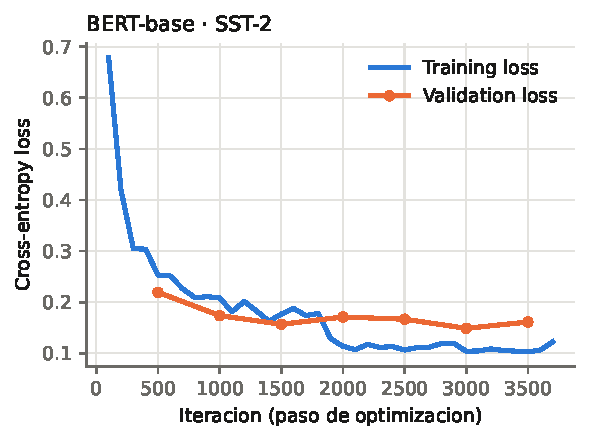
\includegraphics[width=\linewidth]{curvas_bert_sst2.pdf}
  \caption{BERT en SST-2: 37 registros, 2 épocas.}
\end{subfigure}\hfill
\begin{subfigure}[t]{0.48\textwidth}
  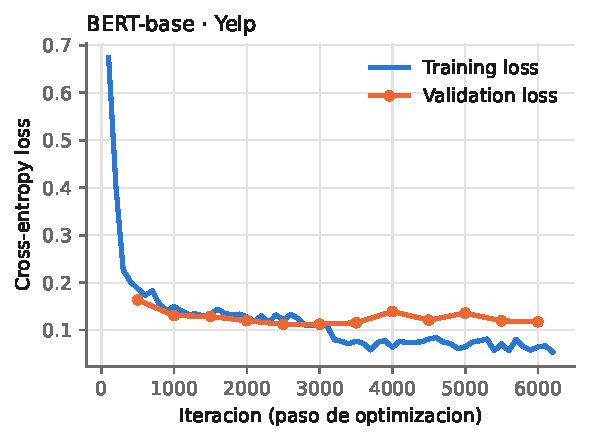
\includegraphics[width=\linewidth]{curvas_bert_yelp.pdf}
  \caption{BERT en Yelp: 62 registros sobre \num{100000} ejemplos.}
\end{subfigure}
\caption{\textit{Cross-entropy loss} de entrenamiento y de validación frente
al número de iteraciones. La validación se evalúa cada 500 pasos, de ahí que
tenga menos puntos. Las curvas de las seis corridas están en
\texttt{results/figures/}.}
\label{fig:curvas}
\end{figure}

Las curvas (Figura~\ref{fig:curvas}) muestran el comportamiento esperado de un
\textit{fine-tuning} corto: la \textit{loss} de entrenamiento cae con rapidez
en los primeros cientos de pasos y después se aplana, mientras la de
validación se estabiliza. En SST-2, el dataset más pequeño, la validación
empieza a separarse del entrenamiento hacia el final de la segunda época
--- el inicio del sobreajuste ---, que es exactamente la razón por la que el
protocolo conserva el \textit{checkpoint} de la mejor época de validación en
lugar del último.

\subsection{Análisis por clase}

El promedio macro oculta dónde se equivoca cada modelo. En AG News, la única
tarea con más de dos clases, los errores no se reparten de forma uniforme
(Tabla~\ref{tab:porclase}).

\begin{table}[h]
\centering
\small
\begin{tabular}{lcccccc}
\toprule
& \multicolumn{3}{c}{\textbf{BERT-base}} & \multicolumn{3}{c}{\textbf{DistilBERT-base}} \\
\cmidrule(lr){2-4}\cmidrule(lr){5-7}
\textbf{Clase} & P & R & F1 & P & R & F1 \\
\midrule
World     & 0,958 & 0,955 & 0,956 & 0,963 & 0,952 & 0,957 \\
Sports    & 0,987 & 0,985 & \best{0,986} & 0,987 & 0,990 & \best{0,988} \\
Business  & 0,927 & 0,903 & 0,915 & 0,924 & 0,905 & 0,915 \\
Sci/Tech  & 0,905 & 0,934 & 0,919 & 0,906 & 0,933 & 0,920 \\
\bottomrule
\end{tabular}
\caption{Desempeño por clase en AG News (\num{1900} ejemplos de test por
clase).}
\label{tab:porclase}
\end{table}

El patrón es idéntico en los dos modelos. \textit{Sports} es casi perfecta
(F1 $\approx 0{,}99$): su vocabulario es distintivo y apenas se solapa con el
resto. \textit{Business} y \textit{Sci/Tech} son las dos peores, y la matriz
de confusión explica por qué: BERT clasifica \num{140} noticias de
\textit{Business} como \textit{Sci/Tech} y \num{90} en sentido contrario;
DistilBERT comete \num{140} y \num{92}. Esos dos flujos concentran la mayor
parte del error de ambos modelos.

La interpretación es que el límite no está en la capacidad del modelo sino en
la tarea: una noticia sobre los resultados trimestrales de una empresa de
semiconductores pertenece legítimamente a las dos categorías. Que BERT, con el
doble de capas, cometa \emph{el mismo} número de confusiones
\textit{Business} $\to$ \textit{Sci/Tech} que DistilBERT es la evidencia más
clara de este informe de que la capacidad adicional no se está
desaprovechando: sencillamente no hay nada más que extraer de esos ejemplos.

\section{Estudio de ablación}
\label{sec:ablation}

\subsection{Diseño}

El estudio se hace sobre DistilBERT y varía dos cosas dejando todo lo demás
fijo: la arquitectura de la cabeza de clasificación y qué parte del
\textit{transformer} se entrena. Son seis configuraciones sobre los tres
datasets, es decir \num{18} corridas.

\begin{table}[h]
\centering
\small
\begin{tabular}{llll}
\toprule
\textbf{Config} & \textbf{Cabeza} & \textbf{\textit{Encoder}} & \textbf{Eje que prueba} \\
\midrule
\texttt{lineal} & $768 \to C$                & entrenable  & menos capas (ninguna oculta) \\
\texttt{h128}   & $768 \to 128 \to C$        & entrenable  & menos neuronas \\
\texttt{h768}   & $768 \to 768 \to C$        & entrenable  & referencia \\
\texttt{h2048}  & $768 \to 2048 \to C$       & entrenable  & más neuronas \\
\texttt{c2}     & $768 \to 512 \to 256 \to C$& entrenable  & más capas \\
\texttt{frz}    & $768 \to 768 \to C$        & \textbf{congelado} & congelar el \textit{transformer} \\
\bottomrule
\end{tabular}
\caption{Las seis configuraciones. $C$ es el número de clases. El diseño cubre
los \emph{dos} sentidos de cada eje --- más y menos capas, más y menos
neuronas --- porque con una sola dirección no se puede afirmar si la métrica
sube o baja de forma monótona.}
\end{table}

\paragraph{Una corrección necesaria en la configuración congelada.} La
configuración \texttt{frz} se entrena con \texttt{lr} $=10^{-3}$ en vez de
$2\times10^{-5}$. El \textit{learning rate} pequeño está pensado para ajustar
pesos ya pre-entrenados; la cabeza sobre un \textit{encoder} congelado se
aprende desde cero y con $2\times10^{-5}$ apenas avanzaría. Sin este ajuste,
\texttt{frz} perdería por el \textit{learning rate} y no por estar congelada,
que es lo que se quiere medir.

\subsection{Resultados}

\begin{figure}[h]
\centering
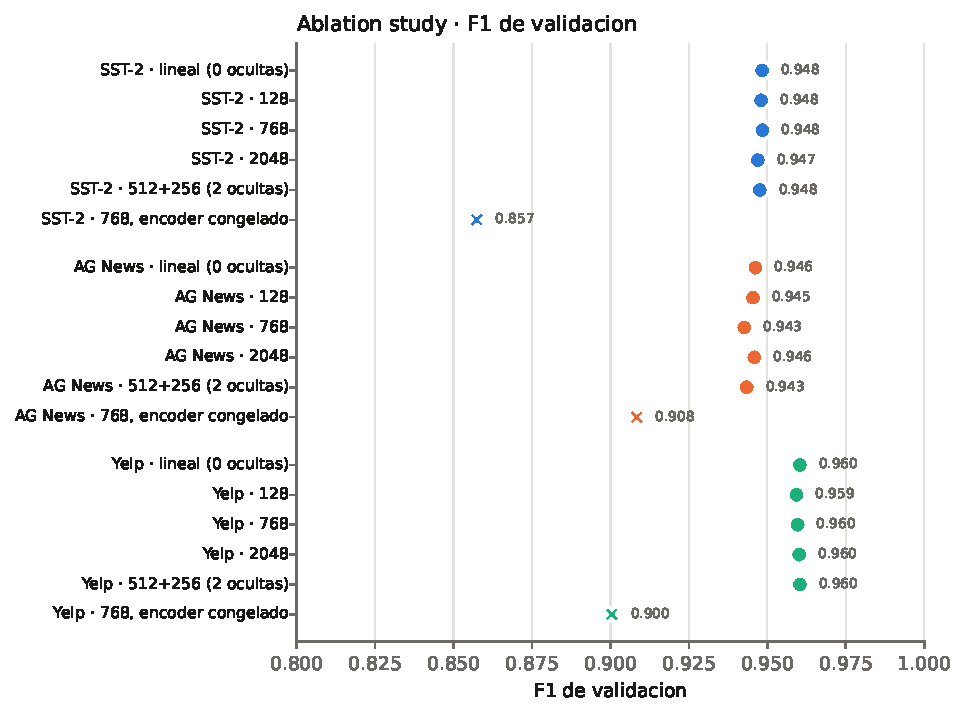
\includegraphics[width=0.86\textwidth]{ablation.pdf}
\caption{F1 de validación de cada configuración, por dataset. El eje llega
desde \num{0,80} a propósito: recortarlo alrededor de las diferencias haría
parecer enormes unas distancias de milésimas. Lo que se ve así es lo que
realmente ocurre --- las cinco cabezas apiladas en el mismo punto y el
\textit{encoder} congelado descolgado ---, y esa es la conclusión del
estudio.}
\label{fig:ablation}
\end{figure}

\begin{table}[h]
\centering
\small
\begin{tabular}{lcccccr}
\toprule
\textbf{Config} & \textbf{SST-2} & \textbf{AG News} & \textbf{Yelp} &
\textbf{Media} & \textbf{Params entren.} & \textbf{Tiempo (min)} \\
\midrule
\texttt{lineal} & 0,9483 & 0,9462 & 0,9603 & \best{0,9516} & 66,4 M & 15,3 \\
\texttt{h2048}  & 0,9470 & 0,9459 & 0,9601 & 0,9510 & 67,9 M & 16,3 \\
\texttt{h128}   & 0,9480 & 0,9454 & 0,9593 & 0,9509 & 66,5 M & 15,9 \\
\texttt{c2}     & 0,9476 & 0,9434 & 0,9604 & 0,9505 & 66,9 M & 15,9 \\
\texttt{h768}   & 0,9485 & 0,9427 & 0,9596 & 0,9503 & 67,0 M & 16,3 \\
\midrule
\texttt{frz}    & 0,8574 & 0,9084 & 0,9005 & 0,8887 & \best{0,6 M}  & \best{6,0} \\
\bottomrule
\end{tabular}
\caption{F1 de \textbf{validación} por configuración, ordenado por la media de
los tres datasets. El tiempo es el total de las tres corridas. La elección se
hace con esta columna; el test no participa.}
\label{tab:ablation}
\end{table}

\subsection{Lectura}

\paragraph{La cabeza de clasificación casi no importa.} Las cinco
configuraciones con el \textit{encoder} entrenable caben en \num{0,0014} de
F1. Un clasificador lineal iguala a un MLP de \num{2048} neuronas y a uno de
dos capas ocultas. Con conjuntos de validación de entre \num{6735} y
\num{20000} ejemplos, esas diferencias están dentro del ruido: ni siquiera el
orden entre ellas es estable --- \texttt{h768} es la mejor en SST-2 y la peor
en media.

Esto tiene una explicación razonable. El \textit{encoder} ya produce, en el
\textit{token} \texttt{[CLS]}, una representación de 768 dimensiones ajustada
a la tarea durante el propio \textit{fine-tuning}. Si esa representación es
linealmente separable, añadir capas por encima no aporta nada: la capacidad
que importa está en el \textit{transformer}, no en el clasificador.

\paragraph{Congelar el \textit{transformer} sí importa, y cuánto depende de la
tarea.} El \textit{encoder} congelado pierde \num{8,4} puntos de F1 en SST-2,
\num{5,8} en Yelp y solo \num{3,4} en AG News. La asimetría es informativa:
clasificar temas de noticias se resuelve casi con las características que
DistilBERT ya trae de fábrica --- es, en buena medida, detección de
vocabulario ---, mientras que detectar sentimiento en frases cortas con
negación y sarcasmo exige que el \textit{encoder} se adapte.

Vale la pena señalar el otro lado del intercambio: \texttt{frz} entrena
\num{0,6}~M de parámetros en lugar de \num{66,4}~M y tarda \num{6,0} minutos
en lugar de \num{15,3}. Para AG News, donde el costo son \num{3,4} puntos de
F1, es un intercambio que podría ser razonable si el presupuesto de
entrenamiento fuera el factor limitante.

\paragraph{Gana \texttt{lineal}, pero no por ser mejor.} Queda empatada con
las demás dentro del ruido, y es la más pequeña y la más rápida de entrenar.
Ante un empate estadístico, la configuración más simple es la elección
defendible.

\section{Eficiencia}
\label{sec:eficiencia}

\subsection{Tamaño y memoria}

Las cifras que no dependen de cómo se mida --- número de parámetros, tamaño
en disco, número de capas --- se resumen en la Tabla~\ref{tab:estatico}. Son
las que justifican por qué se esperaría que DistilBERT fuese más barato; las
dos subsecciones siguientes comprueban si esa expectativa se cumple en
tiempo de ejecución.

\begin{table}[htbp]
\centering
\small
\begin{tabular}{lrrr}
\toprule
 & \textbf{BERT-base} & \textbf{DistilBERT-base} & \textbf{Diferencia} \\
\midrule
Parámetros                    & \num{109483778} & \num{66955010} & $-\SI{38,8}{\percent}$ \\
Tamaño en fp32                & \SI{417,7}{\mega\byte} & \SI{255,4}{\mega\byte} & $-\SI{38,8}{\percent}$ \\
Capas \textit{transformer}    & 12 & 6 & $-\SI{50}{\percent}$ \\
Memoria GPU en inferencia     & $\approx$\SI{1720}{\mega\byte} & $\approx$\SI{1060}{\mega\byte} & $-\SI{38}{\percent}$ \\
Tiempo de entrenamiento (3 datasets) & \SI{29,3}{min} & \SI{16,4}{min} & $-\SI{44}{\percent}$ \\
\bottomrule
\end{tabular}
\caption{Métricas estáticas de eficiencia. La reducción de parámetros
(\SI{38,8}{\percent}) es menor que la de capas (\SI{50}{\percent}) porque la
matriz de \textit{embeddings}, que no se reduce, representa una fracción
importante del total.}
\label{tab:estatico}
\end{table}

\subsection{Por qué la latencia hubo que medirla aparte}

Cada corrida de \textit{fine-tuning} guarda un campo
\texttt{latencia\_ms\_media}, medido al terminar ese entrenamiento y con la
longitud de secuencia de \emph{su} dataset. Esos números \textbf{no son
comparables entre sí}, y al ponerlos juntos producen un resultado absurdo:
BERT en SST-2 marca \SI{3,16}{\milli\second} y DistilBERT en SST-2 marca
\SI{3,50}{\milli\second}. El modelo con el doble de capas saldría ``más
rápido''.

Detectar esto y no reportarlo sin más es parte del resultado. La causa, como
se ve enseguida, es que con \textit{batch} $=1$ la GPU no está calculando sino
esperando a que se lancen los \textit{kernels}, de modo que la medida no
refleja la arquitectura sino el ruido del lanzamiento. La solución fue un
módulo aparte (\texttt{src/benchmark.py}) que mide a los dos modelos en la
\textbf{misma rejilla} de (\textit{batch}, longitud), en la misma GPU y en el
mismo proceso. La latencia no depende de los pesos ajustados sino de la
arquitectura, así que se mide sobre los \textit{checkpoints} pre-entrenados
con entradas sintéticas.

\subsection{Latencia en condiciones controladas}

\begin{table}[h]
\centering
\footnotesize
\setlength{\tabcolsep}{4.5pt}
\begin{tabular}{rr rr c rr c}
\toprule
\textbf{Batch} & \textbf{Long.} & \textbf{BERT} & \textbf{DistilBERT} &
\textbf{Acel.} & \textbf{BERT} & \textbf{DistilBERT} & \textbf{Ratio} \\
 & & (ms) & (ms) & & (MB) & (MB) & mem. \\
\midrule
1  & 64  &   5,56 &  2,60 & \best{2,14$\times$} & 429,9 & 268,6 & 0,62$\times$ \\
1  & 128 &   5,61 &  2,61 & 2,15$\times$ & 433,0 & 271,6 & 0,63$\times$ \\
1  & 256 &   5,11 &  2,74 & 1,86$\times$ & 436,1 & 274,8 & 0,63$\times$ \\
8  & 64  &   7,72 &  4,01 & 1,93$\times$ & 445,9 & 284,5 & 0,64$\times$ \\
8  & 128 &  13,62 &  6,95 & 1,96$\times$ & 461,5 & 299,5 & 0,65$\times$ \\
8  & 256 &  26,59 & 13,39 & 1,99$\times$ & 493,9 & 332,5 & 0,67$\times$ \\
32 & 64  &  24,97 & 12,62 & 1,98$\times$ & 493,9 & 332,5 & 0,67$\times$ \\
32 & 128 &  49,85 & 25,10 & 1,99$\times$ & 559,9 & 398,6 & 0,71$\times$ \\
32 & 256 &  98,10 & 49,25 & 1,99$\times$ & 692,0 & 530,6 & 0,77$\times$ \\
\bottomrule
\end{tabular}
\caption{Latencia y pico de memoria en la misma rejilla (RTX A6000, fp32,
mismo proceso). DistilBERT es \num{2}$\times$ más rápido en los nueve puntos.}
\label{tab:benchmark}
\end{table}

\begin{figure}[h]
\centering
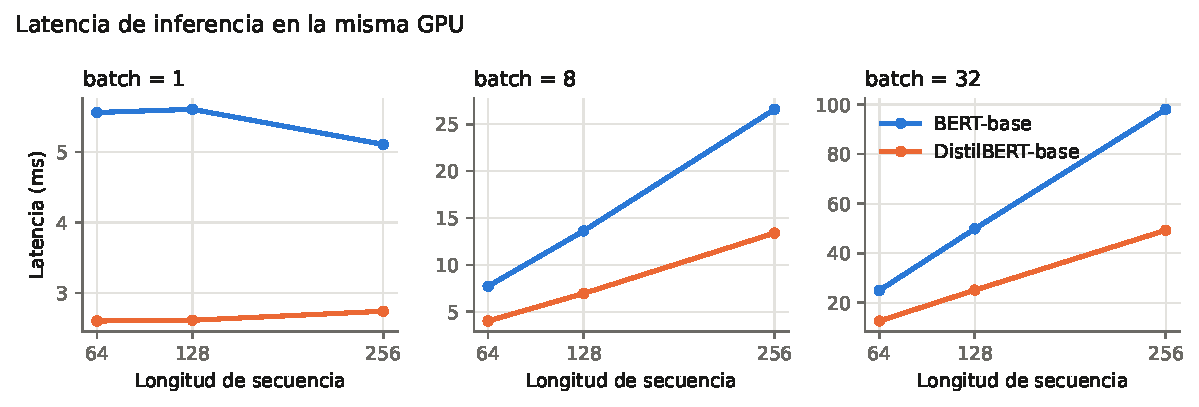
\includegraphics[width=\textwidth]{benchmark_latencia.pdf}
\caption{Latencia frente a longitud de secuencia, un panel por tamaño de
\textit{batch}. Se usan paneles separados en lugar de un solo gráfico porque
las latencias de \textit{batch} 1 y \textit{batch} 32 difieren en un orden de
magnitud y compartir eje aplastaría la curva inferior.}
\label{fig:benchmark}
\end{figure}

Medido así, DistilBERT es \best{2$\times$} más rápido en los nueve puntos de
la rejilla, que es exactamente lo que predice pasar de 12 capas a 6. En
rendimiento, con \textit{batch} 32 y 64 \textit{tokens}: \num{2535} frente a
\num{1282} muestras por segundo.

\paragraph{Los dos regímenes.} La Figura~\ref{fig:benchmark} muestra además
por qué los números por corrida no servían: \textbf{con \textit{batch} $=1$ la
latencia es plana} respecto de la longitud de secuencia: BERT marca
\num{5,56}, \num{5,61} y \num{5,11}~ms para 64, 128 y 256
\textit{tokens}, y DistilBERT \num{2,60}, \num{2,61} y \num{2,74}. Multiplicar por cuatro la longitud no
cuesta nada porque la GPU no está calculando: está esperando a que se lancen
los \textit{kernels}. Solo a partir de \textit{batch} 8 la latencia empieza a
seguir a la longitud, que es cuando la medida significa algo.

La conclusión práctica es que la ventaja de DistilBERT se cobra en los dos
regímenes, pero por motivos distintos: menos \textit{kernels} que lanzar
cuando se sirve petición a petición, y la mitad de cálculo cuando se procesa
por lotes.

\paragraph{La memoria no escala igual que los parámetros.} El ratio de
memoria pasa de \num{0,62}$\times$ con \textit{batch} 1 a \num{0,77}$\times$
con \textit{batch} 32 y 256 \textit{tokens}. Con \textit{batch} pequeño la
memoria está dominada por los pesos, que sí siguen la proporción de
parámetros; al crecer el \textit{batch}, las activaciones pasan a dominar, y
esas dependen de la longitud de secuencia y del tamaño del lote --- iguales
para los dos modelos --- más que del número de capas. En despliegues con
lotes grandes, la ventaja de memoria de DistilBERT se estrecha.

\subsection{Las tres dimensiones a la vez}

\begin{figure}[h]
\centering
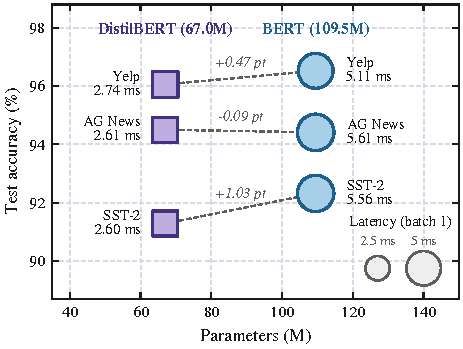
\includegraphics[width=0.78\textwidth]{burbujas_params_acc.pdf}
\caption{Parámetros frente a \textit{accuracy} de test; el área de cada
burbuja es la latencia por muestra. Resume el intercambio completo: cuánto
ocupa, cuánto acierta y cuánto tarda cada combinación de modelo y tarea.}
\label{fig:burbujas}
\end{figure}

La Figura~\ref{fig:burbujas} condensa el argumento del informe. Los puntos de
DistilBERT están a la izquierda (menos parámetros) y en la misma banda
vertical que los de BERT (\textit{accuracy} comparable), con burbujas de área
similar o menor. La distancia vertical entre las dos columnas es pequeña en
todos los casos y prácticamente nula en AG News.

\section{La configuración ganadora en los dos modelos}
\label{sec:mejor}

El último paso aplica la configuración ganadora del estudio de ablación
--- \texttt{lineal}: cabeza $\mathrm{Linear}(768 \to C)$, \textit{encoder}
entrenable --- a BERT y a DistilBERT con el mismo protocolo y los mismos
datos.

\begin{table}[h]
\centering
\small
\begin{tabular}{llccccc r}
\toprule
\textbf{Dataset} & \textbf{Modelo} & \textbf{Accuracy} & \textbf{Precision} &
\textbf{Recall} & \textbf{F1} & \textbf{F1 val.} & \textbf{Train (min)} \\
\midrule
SST-2   & BERT       & \best{0,9289} & 0,9294 & 0,9286 & \best{0,9288} & 0,9541 & 4,2 \\
SST-2   & DistilBERT & 0,9094 & 0,9099 & 0,9091 & 0,9093 & 0,9483 & \best{1,7} \\
\midrule
AG News & BERT       & \best{0,9453} & 0,9456 & 0,9453 & \best{0,9453} & 0,9481 & 9,0 \\
AG News & DistilBERT & 0,9442 & 0,9443 & 0,9442 & 0,9442 & 0,9462 & \best{5,4} \\
\midrule
Yelp    & BERT       & \best{0,9653} & 0,9653 & 0,9653 & \best{0,9653} & 0,9661 & 16,0 \\
Yelp    & DistilBERT & 0,9610 & 0,9610 & 0,9610 & 0,9610 & 0,9603 & \best{8,2} \\
\bottomrule
\end{tabular}
\caption{Configuración \texttt{lineal} en los dos modelos. BERT tiene
\num{109,5}~M de parámetros y DistilBERT \num{66,4}~M.}
\label{tab:mejor}
\end{table}

Con la cabeza lineal, BERT gana en los tres datasets: por \num{1,95} puntos en
SST-2, \num{0,43} en Yelp y \num{0,11} en AG News. Es el mismo patrón de las
corridas base --- la distancia entre los dos modelos depende de la tarea y se
estrecha casi hasta desaparecer en clasificación de temas --- solo que ahora
BERT también gana en AG News, aunque por un margen que sigue dentro del ruido.

\paragraph{Un hallazgo secundario que merece atención.} La cabeza lineal
\emph{mejora} a BERT respecto de su propia corrida base: \num{0,9289} frente a
\num{0,9232} de \textit{accuracy} en SST-2. La corrida base usa la cabeza por
defecto de HuggingFace, que en BERT pasa el \texttt{[CLS]} por un
\textit{pooler} con \texttt{tanh} más \textit{dropout}. Es decir: ese
preprocesado adicional no aporta nada en estas tareas y en SST-2 incluso
estorba. Es coherente con la conclusión del estudio de ablación --- la
capacidad que importa está en el \textit{encoder} --- y llevado un paso más
allá: no solo las capas extra de la cabeza son innecesarias, sino que la
transformación no lineal por defecto puede ser contraproducente.

\section{Limitaciones}
\label{sec:limitaciones}

Cuatro, en orden de importancia para la interpretación de los resultados.

\paragraph{Una sola semilla.} Todas las corridas usan la semilla 42. Sin
repeticiones no hay estimación de la varianza, y por eso a lo largo del
informe las diferencias por debajo de unas décimas se describen como empates
en lugar de como victorias. La afirmación ``la cabeza no importa'' se apoya en
que cinco configuraciones caben en \num{0,0014} de F1, lo cual es consistente
con el ruido esperable pero no es una prueba formal. Repetir con tres o cinco
semillas y reportar media y desviación sería la mejora más valiosa a este
trabajo, y es barata: unas \num{7,5} horas de GPU.

\paragraph{Presupuesto de dos épocas.} El artículo de BERT recomienda entre 2
y 4 épocas para \textit{fine-tuning}. Con 2 se favorece ligeramente al modelo
que converge más rápido, y las curvas de SST-2 sugieren que ahí BERT aún
tenía margen. Es un presupuesto idéntico para los dos modelos, así que no
invalida la comparación, pero sí acota su alcance.

\paragraph{Yelp submuestreado.} Se usan \num{100000} de \num{560000} ejemplos
de train. Los valores absolutos de Yelp están por debajo de lo alcanzable con
el conjunto completo; las diferencias \emph{entre} modelos, que es lo que
interesa, no deberían verse afectadas, porque ambos reciben exactamente el
mismo subconjunto.

\paragraph{Registro de validación incompleto en las corridas base.} Cinco de
las seis corridas base se ejecutaron con una revisión anterior del código de
entrenamiento que no serializaba el resumen de validación por época
(\texttt{desempeno\_val}) en el JSON. La \emph{selección} del mejor
\textit{checkpoint} por F1 de validación sí se aplicó en todas --- está en
las tres revisiones del código ---, y la validación se evaluó durante el
entrenamiento, como demuestran los puntos de \texttt{val\_loss} registrados en
el historial. Lo que falta es solo el registro agregado, motivo por el cual la
Tabla~\ref{tab:desempeno} no incluye columna de F1 de validación y la
Tabla~\ref{tab:mejor}, que proviene de corridas posteriores, sí.

\section{Conclusiones}

\begin{enumerate}

\item \textbf{DistilBERT es la elección por defecto para estas tareas.}
Conserva entre el \SI{98,9}{\percent} y el \SI{99,5}{\percent} de la
\textit{accuracy} de BERT con el \SI{61}{\percent} de los parámetros, el
\SI{62}{\percent} de la memoria y la mitad de la latencia. La pregunta
relevante no es si BERT es mejor --- lo es, por poco --- sino si ese margen
justifica duplicar el costo de inferencia. En AG News no lo justifica en
absoluto; en SST-2, donde la brecha llega a \num{1,95} puntos con la cabeza
lineal, podría hacerlo si la aplicación es sensible a esos puntos.

\item \textbf{La brecha entre los modelos depende de la tarea, no es una
constante.} Va de \num{0,11} puntos en AG News a \num{1,95} en SST-2. La
clasificación de temas se resuelve en buena medida con vocabulario; el
análisis de sentimiento sobre frases cortas, con negación y contraste, exige
la composición que aportan las capas adicionales. Extrapolar un único número
de ``retención de desempeño'' entre tareas sería un error.

\item \textbf{La capacidad que importa está en el \textit{encoder}, no en la
cabeza.} Cinco arquitecturas de cabeza --- de un clasificador lineal a un MLP
de dos capas ocultas --- caben en \num{0,0014} de F1, mientras que congelar el
\textit{transformer} cuesta entre \num{3,4} y \num{8,4} puntos. El corolario
práctico es que el esfuerzo de diseño debe ir a qué se adapta y con qué datos,
no a la arquitectura del clasificador.

\item \textbf{La medición de eficiencia exige condiciones controladas.} La
latencia registrada al final de cada entrenamiento sugería que BERT era más
rápido que DistilBERT en SST-2. Medidos en la misma rejilla, mismo proceso y
misma GPU, DistilBERT resulta \num{2}$\times$ más rápido en los nueve puntos.
La diferencia entre las dos mediciones no está en los modelos sino en el
protocolo, y es un recordatorio de que una métrica de sistema sin condiciones
explícitas no es un resultado.

\item \textbf{Congelar el \textit{encoder} es un intercambio, no un error.}
Entrena \num{0,6}~M de parámetros en lugar de \num{66,4}~M y tarda menos de la
mitad. En AG News el costo es de \num{3,4} puntos de F1, que puede ser
aceptable si el presupuesto de entrenamiento es el factor limitante.

\end{enumerate}


\bibliographystyle{plain}
\bibliography{referencias}

\appendix
\section{Reproducibilidad}
\label{sec:reproducibilidad}

\subsection{Estructura del repositorio}

\begin{lstlisting}
src/
  paths.py          rutas del repo, ancladas a la raiz
  data_adapter.py   carga y normaliza SST-2, AG News y Yelp
  models.py         fabrica de modelos, cabeza configurable y congelado
  train.py          bucle de fine-tuning (escrito a mano, sin Trainer)
  metrics.py        accuracy/precision/recall/F1 + latencia, memoria, tamano
  runs.py           consulta y seleccion de las corridas guardadas
  style.py          paleta y estilo comun de las figuras
  plots.py          figuras del informe (PDF + PNG)
  tables.py         tablas del informe, en Markdown
  benchmark.py      latencia y memoria en una rejilla controlada
scripts/            lanzadores de Slurm
results/
  metrics/          un JSON por corrida (nada se sobrescribe)
  figures/          figuras y tablas generadas por src/plots.py
  logs/             salida de los jobs de Slurm
docs/informe/       este documento
\end{lstlisting}

\subsection{Cómo se reproduce}

\begin{lstlisting}
bash scripts/launch_base.sh distilbert    # 3 corridas base
bash scripts/launch_base.sh bert          # 3 corridas base
CONFIGS=6 sbatch scripts/ablation.sbatch  # 18 corridas del ablation
MODELO=bert CONFIGS=mejor MEJOR="lineal|--head-hidden none" \
    sbatch scripts/ablation.sbatch        # 3 corridas de la ganadora con BERT
sbatch scripts/benchmark.sbatch           # latencia y memoria controladas
python -m src.plots                       # figuras y tablas
\end{lstlisting}

Son \num{24} corridas, unas \num{2,5} horas de GPU en una RTX A6000, en serie
porque la QOS del clúster permite una GPU a la vez.

\subsection{Trazabilidad de las cifras}

Ninguna cifra de este informe se transcribió a mano desde una consola. Cada
entrenamiento escribe un JSON con nombre único
(\texttt{\{modelo\}\_\{tarea\}[\_\{tag\}]\_\{fecha-hora\}.json}) que contiene
las métricas, la configuración completa (\texttt{vars(args)}), el historial de
\textit{loss} por iteración, el desglose por clase y la matriz de confusión.
Nada se sobrescribe nunca. Las tablas y figuras se generan desde esos archivos
con \texttt{python -m src.plots}, que produce además las versiones en Markdown
de cada tabla en \texttt{results/figures/}.

Las etiquetas (\texttt{--tag}) distinguen el propósito de cada corrida:
\texttt{base} para las del informe, \texttt{abl-<config>} para el estudio de
ablación, y \texttt{smoke} o \texttt{pilot} para pruebas y exploraciones, que
quedan excluidas automáticamente de las figuras.

\subsection{Regenerar las figuras sin GPU}

Los JSON están versionados, de modo que todas las figuras y tablas se
reconstruyen sin GPU, sin \texttt{torch} y sin volver a entrenar:

\begin{lstlisting}
pip install matplotlib numpy
python -m src.plots
\end{lstlisting}

La salida es determinista: dos ejecuciones consecutivas producen archivos
idénticos byte a byte, de modo que un archivo marcado como modificado
significa que algún dato cambió.

\subsection{Compilar este informe}

\begin{lstlisting}
cd docs/informe
make              # usa tectonic; genera main.pdf
\end{lstlisting}

Las figuras se leen de \texttt{../../results/figures/} en su versión PDF
(vectorial). El informe nunca contiene una copia de una figura, así que no
puede quedar desincronizado respecto del \textit{pipeline}.


\end{document}
